\documentclass[12pt, a4paper, oneside]{article}\usepackage[]{graphicx}\usepackage[]{color}
%% maxwidth is the original width if it is less than linewidth
%% otherwise use linewidth (to make sure the graphics do not exceed the margin)
\makeatletter
\def\maxwidth{ %
  \ifdim\Gin@nat@width>\linewidth
    \linewidth
  \else
    \Gin@nat@width
  \fi
}
\makeatother

\definecolor{fgcolor}{rgb}{0.345, 0.345, 0.345}
\newcommand{\hlnum}[1]{\textcolor[rgb]{0.686,0.059,0.569}{#1}}%
\newcommand{\hlstr}[1]{\textcolor[rgb]{0.192,0.494,0.8}{#1}}%
\newcommand{\hlcom}[1]{\textcolor[rgb]{0.678,0.584,0.686}{\textit{#1}}}%
\newcommand{\hlopt}[1]{\textcolor[rgb]{0,0,0}{#1}}%
\newcommand{\hlstd}[1]{\textcolor[rgb]{0.345,0.345,0.345}{#1}}%
\newcommand{\hlkwa}[1]{\textcolor[rgb]{0.161,0.373,0.58}{\textbf{#1}}}%
\newcommand{\hlkwb}[1]{\textcolor[rgb]{0.69,0.353,0.396}{#1}}%
\newcommand{\hlkwc}[1]{\textcolor[rgb]{0.333,0.667,0.333}{#1}}%
\newcommand{\hlkwd}[1]{\textcolor[rgb]{0.737,0.353,0.396}{\textbf{#1}}}%

\usepackage{framed}
\makeatletter
\newenvironment{kframe}{%
 \def\at@end@of@kframe{}%
 \ifinner\ifhmode%
  \def\at@end@of@kframe{\end{minipage}}%
  \begin{minipage}{\columnwidth}%
 \fi\fi%
 \def\FrameCommand##1{\hskip\@totalleftmargin \hskip-\fboxsep
 \colorbox{shadecolor}{##1}\hskip-\fboxsep
     % There is no \\@totalrightmargin, so:
     \hskip-\linewidth \hskip-\@totalleftmargin \hskip\columnwidth}%
 \MakeFramed {\advance\hsize-\width
   \@totalleftmargin\z@ \linewidth\hsize
   \@setminipage}}%
 {\par\unskip\endMakeFramed%
 \at@end@of@kframe}
\makeatother

\definecolor{shadecolor}{rgb}{.97, .97, .97}
\definecolor{messagecolor}{rgb}{0, 0, 0}
\definecolor{warningcolor}{rgb}{1, 0, 1}
\definecolor{errorcolor}{rgb}{1, 0, 0}
\newenvironment{knitrout}{}{} % an empty environment to be redefined in TeX

\usepackage{alltt} % Paper size, default font size and one-sided paper
%\graphicspath{{./Figures/}} % Specifies the directory where pictures are stored
%\usepackage[dcucite]{harvard}
\usepackage{amsmath}
\usepackage{setspace}
\usepackage{pdflscape}
\usepackage{rotating}
\usepackage[flushleft]{threeparttable}
\usepackage{multirow}
\usepackage[comma, sort&compress]{natbib}% Use the natbib reference package - read up on this to edit the reference style; if you want text (e.g. Smith et al., 2012) for the in-text references (instead of numbers), remove 'numbers' 
\usepackage{graphicx}
%\bibliographystyle{plainnat}
\bibliographystyle{agsm}
\usepackage[colorlinks = true, citecolor = blue, linkcolor = blue]{hyperref}
%\hypersetup{urlcolor=blue, colorlinks=true} % Colors hyperlinks in blue - change to black if annoying
%\renewcommand[\harvardurl]{URL: \url}
\IfFileExists{upquote.sty}{\usepackage{upquote}}{}
\begin{document}
\title{Stats and Probability Information}
%\author{Rob Hayward\footnote{University of Brighton Business School, Lewes Road, Brighton, BN2 4AT; Telephone 01273 642586.  rh49@brighton.ac.uk}}
\date{\today}
\maketitle
\section*{Continuous and marginal distributions}

The marginal distribution of $x$ in a two-variable distribution is equal to the sum of the joint distribution over $y$. 
\begin{equation}
Pr(X = x) = \sum_y Pr(X = x, Y = y) = \sum_y Pr(X = x|Y = y)Pr(Y = y)
\end{equation}

From \href{http://en.wikipedia.org/wiki/Marginal_distribution}{Wikipedia}

For the continuous case
\begin{equation}
p_X(x) = \int_y p_{X,Y}(x,y)dy = \int_y p_{X|Y}(x|y)p_Y(y)dy
\end{equation}

There are three related distributions:  the marginal, the joint and the conditional. 

\section{Mixture Model}
This is a probabilistic model that relates some random variables to some other variables.  The model has sub-populations. The properties of the sub-population are different from those of the parent. The sub-populations may not be observable.  For example, the distribution of returns may be different in different sub-population or regime. 

A \emph{mixture distribution} is the probability distribution of a random variable  whose values are derived from an underlying set of random variables. The \emph{mixture components} are individual distributions with \emph{mixture weights}.  Even in cases where the mixture comonents have a normal distribution, the mixture distribution is likely to be non-normal. Mixture models are used to understand the sub-population when there is only access to the information about the pooled population. 

The mixture model will be comprised of N random varibles distributed according to K components, with each component belonging to the same distribution. The k mixture weights sum to one. Each component will have parameters (mean and variance in the case of normal distribution).  

The method will try to estimate the all the parameters of the model from the data.  The underlying data is known $(x_i)$; the number of mixture components is set $(K)$; the parameters of the distribution of each mixture component $(\theta_{i=1\dots K})$; mixture weight $(\Phi_{i = 1\dots K})$; $\mathbf{\Phi}$ K-dimensional vector summing to 1; $F(x|\theta)$ probability distribution of observations parameterised on $\theta$; $\alpha$ shared hyperparameter for component weights; $\beta$ shared hyperparameter for mixture weights; $H(\theta|\alpha)$ prior probability distribution of component parameters; 

\section{Adjusted R squared}
\href{http://davegiles.blogspot.ca/2013/05/when-will-adjusted-r-squared-increase.html}{Adjusted R squared} applied a penalty to the basic R squard to account for additional variables.  The equartion is 

\begin{equation}
R_A^2 = 1 - \left [ \frac{(n-1)}{(n-k)} \right ] [1 - R^2]
\end{equation}

Adding a regressor to the equation will increase (reduce)) the $R_A^"$ when the absolute value of the t-statistic is greater (less) than one. Adding a group of regressors to the model will reduce (increase) the $R_A^"$ when the absolute value of the F-statistic is greater than one.  

Proof \href{http://davegiles.blogspot.com/2014/04/proof-of-result-about-adjusted.html}{http://davegiles.blogspot.com/2014/04/proof-of-result-about-adjusted.html}


\section{Monte Carlo Simulation}
This comes from \href{http://blog.revolutionanalytics.com/2014/04/quantitative-finance-applications-in-r-5.html}{Revoluitionary Analytics}.  The analysis is in annual terms.  

\begin{equation}
\mu \Delta t + \sigma Z \sqrt{\Delta t}
\end{equation}

where $\mu$ is the drift or average annual return, Z is a standard Normal random variable, t is measured in years so for monthly returns $\Delta t$ equals $\frac{1}{12}$.

\begin{knitrout}
\definecolor{shadecolor}{rgb}{0.969, 0.969, 0.969}\color{fgcolor}\begin{kframe}
\begin{alltt}
\hlstd{n} \hlkwb{<-} \hlnum{10000}
\hlcom{# Fixing the seed gives us a consistent set of simulated returns}
\hlkwd{set.seed}\hlstd{(}\hlnum{106}\hlstd{)}
\hlstd{z} \hlkwb{<-} \hlkwd{rnorm}\hlstd{(n)}  \hlcom{# mean = 0 and sd = 1 are defaults}
\hlstd{mu} \hlkwb{<-} \hlnum{0.1}
\hlstd{sd} \hlkwb{<-} \hlnum{0.15}
\hlstd{delta_t} \hlkwb{<-} \hlnum{0.25}
\hlcom{# apply to expression (*) above}
\hlstd{qtr_returns} \hlkwb{<-} \hlstd{mu} \hlopt{*} \hlstd{delta_t} \hlopt{+} \hlstd{sd} \hlopt{*} \hlstd{z} \hlopt{*} \hlkwd{sqrt}\hlstd{(delta_t)}
\hlkwd{hist}\hlstd{(qtr_returns,} \hlkwc{breaks} \hlstd{=} \hlnum{100}\hlstd{,} \hlkwc{col} \hlstd{=} \hlstr{"green"}\hlstd{)}
\end{alltt}
\end{kframe}
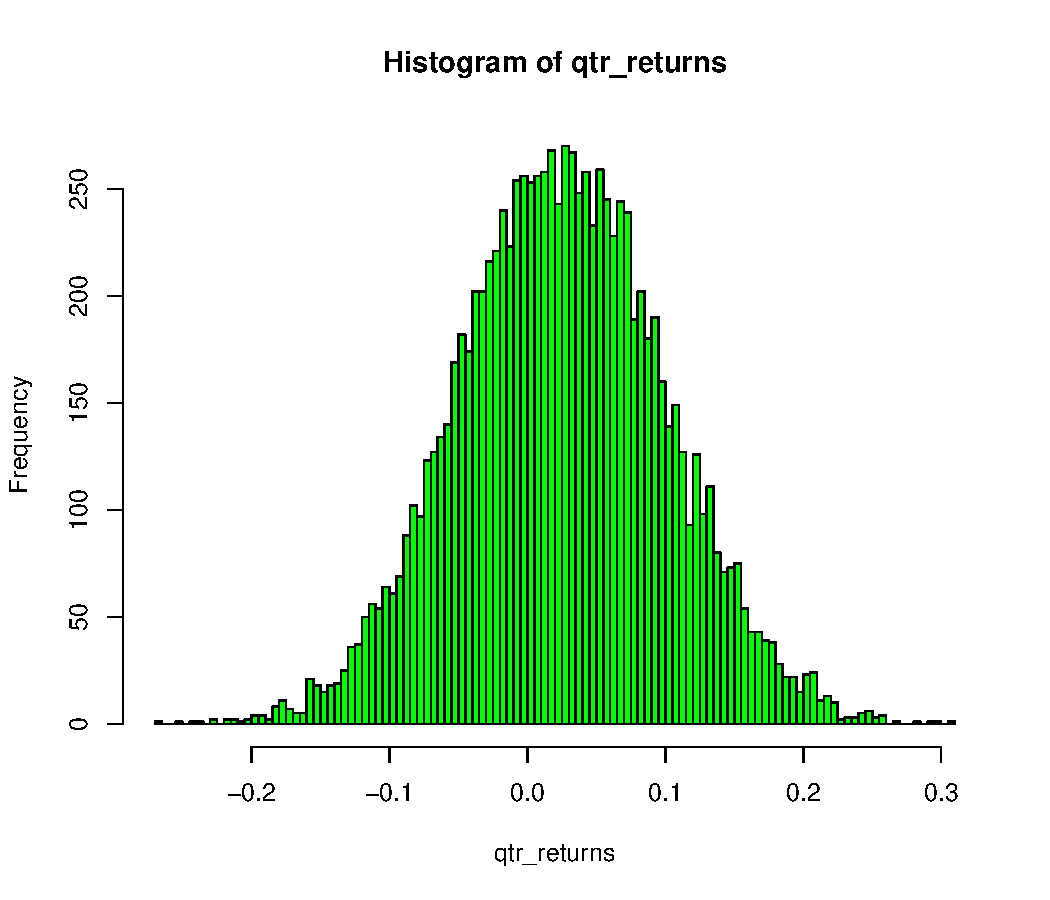
\includegraphics[width=\maxwidth]{figure/MC} 

\end{knitrout}


Now the descriptive statistics can be uncovered from the simulated results. 
\begin{knitrout}
\definecolor{shadecolor}{rgb}{0.969, 0.969, 0.969}\color{fgcolor}\begin{kframe}
\begin{alltt}
\hlstd{stats} \hlkwb{<-} \hlkwd{c}\hlstd{(}\hlkwd{mean}\hlstd{(qtr_returns)} \hlopt{*} \hlnum{4}\hlstd{,} \hlkwd{sd}\hlstd{(qtr_returns)} \hlopt{*} \hlnum{2}\hlstd{)}  \hlcom{# sqrt(4)}
\hlkwd{names}\hlstd{(stats)} \hlkwb{<-} \hlkwd{c}\hlstd{(}\hlstr{"mean"}\hlstd{,} \hlstr{"volatility"}\hlstd{)}
\hlstd{stats}
\end{alltt}
\begin{verbatim}
##       mean volatility 
##    0.09901    0.14976
\end{verbatim}
\end{kframe}
\end{knitrout}

This is the basic model.  It would also be possible to simulate two variables and to include some relationship between the two in the analysis.  It would also be possible to simulate an asset in two different regimes. A Monte-Carlo Markov Model (MCMM) would require another set of $\mu$ and $\sigma$ inputs as well as a transition matrix of the probabilities that there is a switch from one regime to another. 
 
\section{Generalised Lambda Distribution}
This is from \href{http://blog.revolutionanalytics.com/2014/02/quantitative-finance-applications-in-r-4-using-the-generalized-lambda-distribution-to-simulate-market-returns.html}{Revolutionary Analytics}.  The four parameters $\lambda_1$, $\lambda_2$, $\lambda_3$ and $\lambda_4$ indicate the location, scale, skew and kurtosis of the distribution. 

\begin{knitrout}
\definecolor{shadecolor}{rgb}{0.969, 0.969, 0.969}\color{fgcolor}\begin{kframe}
\begin{alltt}
\hlkwd{require}\hlstd{(GLDEX)}
\hlkwd{require}\hlstd{(quantmod)}
\hlkwd{getSymbols}\hlstd{(}\hlstr{"SPY"}\hlstd{,} \hlkwc{from} \hlstd{=} \hlstr{"1994-02-01"}\hlstd{)}
\end{alltt}
\begin{verbatim}
## [1] "SPY"
\end{verbatim}
\begin{alltt}
\hlstd{SPY.Close} \hlkwb{<-} \hlstd{SPY[,} \hlnum{4}\hlstd{]}  \hlcom{# Closing prices}
\hlstd{SPY.vector} \hlkwb{<-} \hlkwd{as.vector}\hlstd{(SPY.Close)}
\hlcom{# Calculate log returns}
\hlstd{sp500} \hlkwb{<-} \hlkwd{diff}\hlstd{(}\hlkwd{log}\hlstd{(SPY.vector),} \hlkwc{lag} \hlstd{=} \hlnum{1}\hlstd{)}
\hlstd{sp500} \hlkwb{<-} \hlstd{sp500[}\hlopt{-}\hlnum{1}\hlstd{]}  \hlcom{# Remove the NA in the first position}
\hlcom{# Set normalise='Y' so that kurtosis is calculated with reference to}
\hlcom{# kurtosis = 0 under Normal distribution}
\hlkwd{fun.moments.r}\hlstd{(sp500,} \hlkwc{normalise} \hlstd{=} \hlstr{"Y"}\hlstd{)}
\end{alltt}
\begin{verbatim}
##       mean   variance   skewness   kurtosis 
##  0.0002633  0.0001532 -0.0960976  9.5131553
\end{verbatim}
\end{kframe}
\end{knitrout}

Now fit the GLD with the function fun.data.fit.mm. There are warnings but these can be ignored. 

\begin{knitrout}
\definecolor{shadecolor}{rgb}{0.969, 0.969, 0.969}\color{fgcolor}\begin{kframe}
\begin{alltt}
\hlstd{spLambdaDist} \hlkwb{=} \hlkwd{fun.data.fit.mm}\hlstd{(sp500)}
\hlstd{spLambdaDist}
\end{alltt}
\begin{verbatim}
##            RPRS     RMFMKL
## [1,]  3.846e-04   0.000321
## [2,] -4.228e+01 203.501581
## [3,] -1.675e-01  -0.169657
## [4,] -1.640e-01  -0.161483
\end{verbatim}
\begin{alltt}
\hlkwd{fun.plot.fit}\hlstd{(}\hlkwc{fit.obj} \hlstd{= spLambdaDist,} \hlkwc{data} \hlstd{= sp500,} \hlkwc{nclass} \hlstd{=} \hlnum{100}\hlstd{,} \hlkwc{param} \hlstd{=} \hlkwd{c}\hlstd{(}\hlstr{"rs"}\hlstd{,}
    \hlstr{"fmkl"}\hlstd{),} \hlkwc{xlab} \hlstd{=} \hlstr{"Returns"}\hlstd{)}
\end{alltt}
\end{kframe}
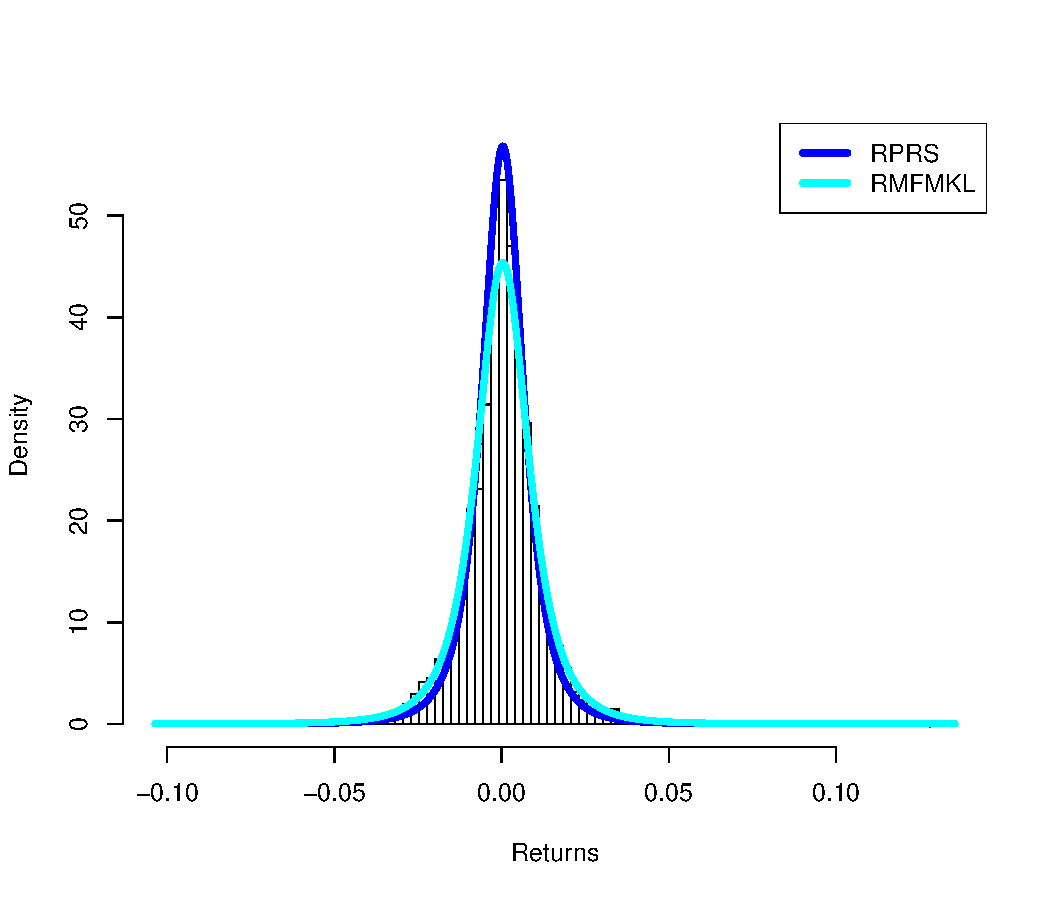
\includegraphics[width=\maxwidth]{figure/GLD} 

\end{knitrout}

Now it is possible to generrate simualted results using the function rgl(). Lambdas need to be identified. 
\begin{knitrout}
\definecolor{shadecolor}{rgb}{0.969, 0.969, 0.969}\color{fgcolor}\begin{kframe}
\begin{alltt}
\hlstd{lambda_params_rs} \hlkwb{<-} \hlstd{spLambdaDist[,} \hlnum{1}\hlstd{]}
\hlstd{lambda1_rs} \hlkwb{<-} \hlstd{lambda_params_rs[}\hlnum{1}\hlstd{]}
\hlstd{lambda2_rs} \hlkwb{<-} \hlstd{lambda_params_rs[}\hlnum{2}\hlstd{]}
\hlstd{lambda3_rs} \hlkwb{<-} \hlstd{lambda_params_rs[}\hlnum{3}\hlstd{]}
\hlstd{lambda4_rs} \hlkwb{<-} \hlstd{lambda_params_rs[}\hlnum{4}\hlstd{]}
\hlstd{lambda_params_fmkl} \hlkwb{<-} \hlstd{spLambdaDist[,} \hlnum{2}\hlstd{]}
\hlstd{lambda1_fmkl} \hlkwb{<-} \hlstd{lambda_params_fmkl[}\hlnum{1}\hlstd{]}
\hlstd{lambda2_fmkl} \hlkwb{<-} \hlstd{lambda_params_fmkl[}\hlnum{2}\hlstd{]}
\hlstd{lambda3_fmkl} \hlkwb{<-} \hlstd{lambda_params_fmkl[}\hlnum{3}\hlstd{]}
\hlstd{lambda4_fmkl} \hlkwb{<-} \hlstd{lambda_params_fmkl[}\hlnum{4}\hlstd{]}
\end{alltt}
\end{kframe}
\end{knitrout}

Now generate simulations of each variety. 

There are problems with the rgl function.  I am not sure what this does.  It is 10 million simulations.  I think that the rgl just uses extra hardware to make the change. It may be useful to re-do this last section using a different method. 
\begin{knitrout}
\definecolor{shadecolor}{rgb}{0.969, 0.969, 0.969}\color{fgcolor}\begin{kframe}
\begin{alltt}
\hlkwd{require}\hlstd{(gld)}
\end{alltt}


{\ttfamily\noindent\itshape\color{messagecolor}{\#\# Loading required package: gld}}\begin{alltt}
\hlkwd{require}\hlstd{(GLDEX)}
\end{alltt}


{\ttfamily\noindent\itshape\color{messagecolor}{\#\# Loading required package: GLDEX\\\#\# Loading required package: cluster\\\#\# \\\#\# Attaching package: 'GLDEX'\\\#\# \\\#\# The following objects are masked from 'package:gld':\\\#\# \\\#\#\ \ \ \  dgl, pgl, qdgl, qgl, rgl, starship, starship.adaptivegrid,\\\#\#\ \ \ \  starship.obj}}\begin{alltt}
\hlcom{# RS version:}
\hlkwd{set.seed}\hlstd{(}\hlnum{100}\hlstd{)}  \hlcom{# Set seed to obtain a reproducible set}
\hlstd{rs_sample} \hlkwb{<-} \hlkwd{rgl}\hlstd{(}\hlkwc{n} \hlstd{=} \hlnum{1e+07}\hlstd{,} \hlkwc{lambda1} \hlstd{= lambda1_rs,} \hlkwc{lambda2} \hlstd{= lambda2_rs,} \hlkwc{lambda3} \hlstd{= lambda3_rs,}
    \hlkwc{lambda4} \hlstd{= lambda4_rs,} \hlkwc{param} \hlstd{=} \hlstr{"rs"}\hlstd{)}
\hlcom{# Moments of simulated returns using RS method:}
\hlkwd{fun.moments.r}\hlstd{(rs_sample,} \hlkwc{normalise} \hlstd{=} \hlstr{"Y"}\hlstd{)}
\end{alltt}
\begin{verbatim}
##       mean   variance   skewness   kurtosis 
##  2.633e-04  9.774e-05 -1.043e-01  9.955e+00
\end{verbatim}
\begin{alltt}
\hlcom{# Moments calculated from market data:}
\hlkwd{fun.moments.r}\hlstd{(sp500,} \hlkwc{normalise} \hlstd{=} \hlstr{"Y"}\hlstd{)}
\end{alltt}
\begin{verbatim}
##       mean   variance   skewness   kurtosis 
##  0.0002633  0.0001532 -0.0960976  9.5131553
\end{verbatim}
\begin{alltt}
\hlcom{# FKML version:}
\hlkwd{set.seed}\hlstd{(}\hlnum{100}\hlstd{)}  \hlcom{# Set seed to obtain a reproducible set}
\hlstd{fmkl_sample} \hlkwb{<-} \hlkwd{rgl}\hlstd{(}\hlkwc{n} \hlstd{=} \hlnum{1e+05}\hlstd{,} \hlkwc{lambda1} \hlstd{= lambda1_fmkl,} \hlkwc{lambda2} \hlstd{= lambda2_fmkl,}
    \hlkwc{lambda3} \hlstd{= lambda3_fmkl,} \hlkwc{lambda4} \hlstd{= lambda4_fmkl,} \hlkwc{param} \hlstd{=} \hlstr{"fmkl"}\hlstd{)}
\hlcom{# Moments of simulated returns using FMKL method:}
\hlkwd{fun.moments.r}\hlstd{(fmkl_sample,} \hlkwc{normalise} \hlstd{=} \hlstr{"Y"}\hlstd{)}
\end{alltt}
\begin{verbatim}
##       mean   variance   skewness   kurtosis 
##  0.0002403  0.0001547 -0.0862244  8.5839659
\end{verbatim}
\begin{alltt}
\hlcom{# Moments calculated from market data:}
\hlkwd{fun.moments.r}\hlstd{(sp500,} \hlkwc{normalise} \hlstd{=} \hlstr{"Y"}\hlstd{)}
\end{alltt}
\begin{verbatim}
##       mean   variance   skewness   kurtosis 
##  0.0002633  0.0001532 -0.0960976  9.5131553
\end{verbatim}
\end{kframe}
\end{knitrout}

Compare the moments to the S\&P500 market data
\begin{knitrout}
\definecolor{shadecolor}{rgb}{0.969, 0.969, 0.969}\color{fgcolor}\begin{kframe}
\begin{alltt}
\hlkwd{fun.moments.r}\hlstd{(rs_sample,} \hlkwc{normalise} \hlstd{=} \hlstr{"Y"}\hlstd{)}
\end{alltt}
\begin{verbatim}
##       mean   variance   skewness   kurtosis 
##  2.633e-04  9.774e-05 -1.043e-01  9.955e+00
\end{verbatim}
\begin{alltt}
\hlkwd{fun.moments.r}\hlstd{(sp500,} \hlkwc{normalise} \hlstd{=} \hlstr{"Y"}\hlstd{)}
\end{alltt}
\begin{verbatim}
##       mean   variance   skewness   kurtosis 
##  0.0002633  0.0001532 -0.0960976  9.5131553
\end{verbatim}
\begin{alltt}
\hlkwd{fun.moments.r}\hlstd{(fmkl_sample,} \hlkwc{normalise} \hlstd{=} \hlstr{"Y"}\hlstd{)}
\end{alltt}
\begin{verbatim}
##       mean   variance   skewness   kurtosis 
##  0.0002403  0.0001547 -0.0862244  8.5839659
\end{verbatim}
\begin{alltt}
\hlkwd{fun.moments.r}\hlstd{(sp500,} \hlkwc{normalise} \hlstd{=} \hlstr{"Y"}\hlstd{)}
\end{alltt}
\begin{verbatim}
##       mean   variance   skewness   kurtosis 
##  0.0002633  0.0001532 -0.0960976  9.5131553
\end{verbatim}
\end{kframe}
\end{knitrout}

\end{document}
